\documentclass{ieeeaccess}
\usepackage{cite}
\usepackage{amsmath,amssymb,amsfonts}
\usepackage{graphicx}
\usepackage{booktabs}
\usepackage{textcomp}
\usepackage{url}
\graphicspath{{figs/}}

\newcommand{\rzero}{r_0}
\newcommand{\tauc}{\tau_{\mathrm{corr}}}

\begin{document}
\history{Date of publication xxxx 00, 0000, date of current version xxxx 00, 0000.}
\doi{10.1109/ACCESS.2026.DOI}

\title{Overclocking the p-bit: Stochastic Binary Neural Network Inference with Autocorrelated sMTJ Randomness}

\author{\uppercase{Manan Gupta}\authorrefmark{1}}
\address[1]{The Harker School, San Jose, CA 95129 USA (e-mail: mnn@yogins.com)}

\corresp{Corresponding author: Manan Gupta (e-mail: mnn@yogins.com).}

\begin{abstract}
Stochastic magnetic tunnel junctions (sMTJs) produce physically random bits
at about 0.03\,pJ per bit, five to six orders of magnitude less energy than
software pseudorandom generation. They are therefore promising entropy
sources for probabilistic-bit (p-bit) neural hardware. The usual design rule
requires a sampling interval of at least twice the mean dwell time so that
successive bits are uncorrelated. Existing systems follow this rule, but its
application-level cost is unknown. We treat the ratio of sampling interval to
correlation time as a continuous design parameter and simulate stochastic
binary-network classification on MNIST and Fashion-MNIST using telegraph
sMTJ neurons. The operating mode matters more than the sampling rate. In
settle mode, a measured per-input relaxation of about four correlation times
makes accuracy nearly independent of rate: with 32 samples, sampling
$200\times$ faster than the rule costs less than 0.7 percentage points. In
continuous streaming, however, stale states carry activations from one input
to the next, and single-sample accuracy falls to chance. Device-to-device
dwell-time dispersion does not solve this problem. At a fixed central
fluctuation rate, it modestly reduces accuracy. The more consequential choice
is the population statistic held fixed in fabrication: fixing mean rather
than median correlation time multiplies every device rate by
$e^{\sigma_\Delta^2/2}$, a $3\times$ shift at $\sigma_\Delta=1.5\,k_BT$.
Finally, correlation-aware training, which backpropagates through
correlated activations, recovers much of the streaming loss (28\% to 85\%
at the harshest setting) for a 3.3-point cost at nominal speed. It extends
the accuracy--throughput Pareto frontier to $2\times$ the rule-compliant
optimum at 97\% accuracy, $4\times$ at 95\%, and $8\times$ at 90\%.
\end{abstract}

\begin{keywords}
probabilistic computing, p-bit, stochastic magnetic tunnel junction,
binarized neural networks, random telegraph noise, energy-efficient inference
\end{keywords}

\titlepgskip=-21pt

\maketitle

\section{Introduction}
\IEEEPARstart{G}{enerating} randomness is expensive on conventional
hardware: pseudorandom generation at Gb/s rates costs about 30\,nJ per bit
on CPUs and 3\,nJ per bit on GPUs~\cite{sun2026superparamagnetic}. A
stochastic magnetic tunnel junction (sMTJ) is a nanomagnet whose free layer
thermally switches between two states. It produces physically random bits at
about 0.03\,pJ per bit~\cite{sun2026superparamagnetic}. This roughly
$10^6$-fold energy gap motivates probabilistic-bit (p-bit)
computing~\cite{camsari2017stochastic,kaiser2021probabilistic}. In a p-bit
system, the sMTJ is the stochastic neuron rather than a separate random-bit
generator: an input current biases its time-averaged state to
$\langle m \rangle = \tanh(I)$~\cite{camsari2017stochastic}, the activation
used by stochastic binary neural networks (SBNNs).

An sMTJ also has its own switching timescale. Reading it faster than it
switches returns repeated, stale states rather than independent samples.
Daniels \emph{et al.}\ found that adjacent samples become uncorrelated only
when the sampling interval exceeds about twice the \emph{mean dwell time}
$\tau_d$~\cite{daniels2020energy}. This ``$2\tau$ rule'' is commonly treated
as a hard constraint. Demonstrated systems oversample the relaxation time by
large factors~\cite{singh2024cmos}, and random-bit quality is assessed with
statistical test suites~\cite{vodenicarevic2017low,sun2026superparamagnetic}.
Prior work has examined the timing trade for sampling machines: autonomous
Ising machines require synapses to respond faster than neuron fluctuations
\cite{sutton2020autonomous}, and in situ Boltzmann learning requires a
learning time constant longer than the MTJ fluctuation time
\cite{kaiser2022hardware}. What remains unclear is the application-level
cost. No published study continuously maps sampling ratio to feedforward
classification accuracy, separates the operating modes in which correlation
matters, or tests how much training can recover. This paper addresses those
questions with three contributions:

\begin{itemize}
\item \textbf{Operating mode matters more than rate.} We model sMTJ
neurons as input-biased telegraph processes with an exact discrete-time
propagator and the stationary p-bit activation law. We sweep
$\rzero=\Delta t/\tauc(0)$ across four decades. In settle mode, we measure
rather than assume the required relaxation interval: a settle of about
$4\tauc$ makes classification nearly rate-independent. At $\rzero=0.02$,
which is $200\times$ faster than the rule, 32-sample accuracy falls only
from 97.7\% to 97.1\%. In continuous streaming, stale activation states
cross input boundaries and single-sample accuracy reaches chance (10\%)
below $\rzero\approx0.05$. Increasing samples by $32\times$ shifts this
threshold by roughly one order of magnitude in $\rzero$. The same collapse
appears, and is worse, for a bias-independent-rate variant, indicating that
the cause is generic staleness rather than the Arrhenius model.
\item \textbf{The centering convention matters more than dispersion.}
Whether device-to-device dwell-time dispersion appears helpful or harmful
depends on the population statistic held fixed during fabrication. Because
dwell time varies exponentially with barrier offset, fixing the \emph{mean}
correlation time instead of the \emph{median} device multiplies every rate
by $e^{\sigma_\Delta^2/2}$, or $3.1\times$ at
$\sigma_\Delta=1.5\,k_BT$. This uniform rate shift explains nearly all of
the apparent recovery from 72\% to 94\% at $\rzero=0.05$. At matched
central rates, dispersion costs 1--5 accuracy points because the slow tail
dominates. Device specifications should therefore state the central
fluctuation rate explicitly; dispersion around it is a smaller effect.
\item \textbf{Correlation-aware training extends the Pareto frontier.}
Training with activations sampled from the correlated telegraph process,
with state carried across minibatches, recovers most of the streaming loss:
at $\rzero=0.02$ and $T{=}32$, accuracy rises from 28\% to 85\%. This
costs 3.3 points at nominal speed; a milder version costs 1.2 points. When
throughput includes the measured $\approx4\tauc$ settle time per input,
the frontier reaches $2\times$ the best rule-compliant operating point at
97\% accuracy, $4\times$ at 95\%, and $8\times$ at 90\%. The two larger
gains come from correlation-aware training.
\end{itemize}

\section{Background and Related Work}
\label{sec:related}

\subsection{p-bits and sMTJ entropy sources}
A p-bit produces $m=\mathrm{sgn}\{\mathrm{rand}(-1,1)+\tanh I\}$ on each
query, so its mean is $\langle m\rangle=\tanh(I)$
\cite{camsari2017stochastic}. Superparamagnetic MTJs with barriers near
$1.4\,k_BT$~\cite{sun2026superparamagnetic} implement this behavior
natively. Their dwell time is $\tau=\tau_0e^{\Delta/k_BT}$, where
$\tau_0\approx10\,\mathrm{ps}$--$1\,\mathrm{ns}$
\cite{camsari2017stochastic}. Reported fluctuation times range from
2--5\,ns autocorrelation in easy-plane devices
\cite{safranski2021nanosecond} and nanosecond-scale telegraph noise in
in-plane junctions~\cite{hayakawa2021nanosecond}, to the slower devices
used in early p-bit demonstrations~\cite{borders2019integer}. One early
system operated with millisecond-scale fluctuations. A recent heterogeneous
CMOS-plus-nanomagnet system samples a roughly 20\,ms relaxation time at
$40\times$ the rate~\cite{singh2024cmos}.

\subsection{Randomness quality, sampling, and neural inference}
Robustness studies of MTJ neural hardware have mainly examined \emph{static}
imperfections, including sigmoid distortion from process variation
\cite{wood2020modular,zand2018composable} and parameter spread in fabricated
arrays with compensation~\cite{zhang2025automatic}. Work on sMTJ generators
typically evaluates random-bit streams with NIST tests
\cite{vodenicarevic2017low,sun2026superparamagnetic}. Other studies show
that PRNG quality can have a threshold effect on MNIST training
\cite{prng2025quality}, and that measured sMTJ bitstreams can support
stochastic-computing inference despite their native correlation
\cite{spintronicSC2025}. Bit-level correlation has long been a primary
variable in stochastic computing~\cite{alaghi2013survey,alaghi2013exploiting}.
Recent work also finds that averaging stochastic binary activations, and
training through that average, improves p-bit network accuracy
\cite{ghantasala2026sampling}. The theory is well established:
autocorrelation reduces the effective sample size of a Monte Carlo average
\cite{sokal1997monte}, and spiking networks can have an optimal noise level
\cite{timcheck2022optimal}. We study the missing combination: a continuous
sampling-ratio sweep mapped to feedforward classification accuracy across
operating modes, variability models, and training regimes.

\section{Model}
\label{sec:model}

\subsection{The sMTJ neuron as a biased telegraph process}
Each hidden unit is a two-state fluctuator $s \in \{-1,+1\}$ with
input-modulated Arrhenius escape rates
\begin{equation}
k_{-\to+} = f\, e^{+I}, \qquad k_{+\to-} = f\, e^{-I},
\label{eq:rates}
\end{equation}
where $I$ is the dimensionless synaptic input and $f = f_0 e^{-\delta
\Delta}$ the device attempt rate with per-device barrier offset
$\delta\Delta$ (in $k_BT$). The stationary law is
\begin{equation}
P(s{=}{+}1) = \frac{k_{-\to+}}{k_{-\to+}+k_{+\to-}} = \frac{1+\tanh I}{2}
\equiv p,
\label{eq:peq}
\end{equation}
because $\langle m\rangle=\tanh I$ and $\langle m\rangle=2P(+1)-1$
\cite{camsari2017stochastic}. Thus each neuron has the p-bit activation
law at every operating point; changing the sampling rate changes only its
temporal structure. The correlation time is
\begin{equation}
\tauc(I) = \frac{1}{k_{-\to+}+k_{+\to-}} = \frac{1}{2f\cosh I},
\label{eq:tauc}
\end{equation}
so strongly biased neurons decorrelate faster. Correlation time and mean
dwell time are different quantities. At $I{=}0$,
$\tau_d=1/f=2\tauc$, so the Daniels $2\tau_d$ rule
\cite{daniels2020energy} is $\rzero\geq4$ in our units. At nonzero bias,
the occupancy-weighted dwell-to-correlation ratio grows as $2\cosh2I$;
the corresponding dwell-time rule is therefore stricter for driven
devices. We quote the rule at $I{=}0$:
\begin{equation}
\rzero \;=\; 2 f_0 \Delta t \;=\; \Delta t/\tauc(0)\big|_{\delta\Delta=0}.
\end{equation}
We assume each input remains constant during an inter-query interval, as in
sample-and-hold operation between clocked layers. The exact two-state
propagator then has no discretization error:
\begin{equation}
P(s_{t+\Delta t}{=}{+}1 \mid s_t) = p + \left(\mathbb{1}[s_t{=}{+}1] -
p\right) e^{-\Delta t/\tauc},
\label{eq:propagator}
\end{equation}
with $\Delta t/\tauc = \rzero e^{-\delta\Delta}\cosh I$.

Equation~\eqref{eq:rates} describes the energy-tilt behavior of
barrier-type devices in the Arrhenius regime. Easy-plane sMTJs are designed
to have a fluctuation rate that changes little with bias
\cite{safranski2021nanosecond,sun2026superparamagnetic}. We therefore also
simulate a \textbf{bias-independent-rate variant}: its total rate is fixed
at $2f$, so $\Delta t/\tauc=\rzero e^{-\delta\Delta}$ while the stationary
law remains the same. Device variability is modeled by a barrier offset
$\delta\Delta\sim\mathcal{N}(\mu,\sigma_\Delta^2)$ that is fixed for each
chip. Since dwell time depends exponentially on $\delta\Delta$, the choice
of $\mu$ determines the population statistic held fixed as
$\sigma_\Delta$ grows. Setting $\mu=0$ fixes the \emph{median} device and
makes the mean correlation time grow as $e^{\sigma_\Delta^2/2}$. Setting
$\mu=-\sigma_\Delta^2/2$ fixes the \emph{mean} correlation time. We report
both cases because either can describe a fabrication corner. Neither changes
the stationary firing probability, which isolates the temporal effect of
variability from static sigmoid distortion
\cite{wood2020modular,zand2018composable,zhang2025automatic}. Our model
omits read disturb, $1/f$ resistance noise, temperature drift, and behavior
outside the two-state telegraph regime
\cite{safranski2021nanosecond,hayakawa2021nanosecond}.

\begin{figure}[t]
\centering
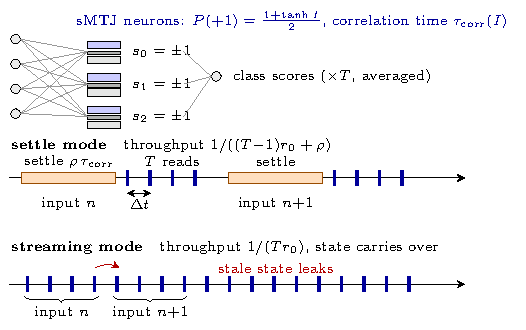
\includegraphics[width=\columnwidth]{fig_modes}
\caption{SBNN with sMTJ neurons (top) and the two operating modes
(bottom). Settle mode pays $\rho\,\tauc$ of relaxation per input; in
streaming mode devices are never idle and the previous input's activation
pattern persists in the device states.}
\label{fig:modes}
\end{figure}

\subsection{Operating modes: settle vs.\ streaming}
\label{sec:modes}
In \textbf{settle mode}, which models batch-style inference, an input is
applied and the device relaxes for $t_s=\rho\,\tauc(0)$ before the first of
$T$ reads. Consecutive reads are separated by $\Delta t$. A device left idle
for a long time equilibrates to $p=1/2$, not to the stationary distribution
of the next input. In continuous operation, its initial state is instead
the final state from the previous input. In both cases, settling moves the
device toward $p_{\mathrm{eq}}(I)$ with time constant $\tauc(I)$. Starting
from idle, the first read has residual bias
$-\tfrac{1}{2}\tanh(I)e^{-\rho\cosh I}$. We simulate this relaxation from
the actual preceding state and sweep $\rho$ to measure the needed interval.
We charge the settle time to throughput: settle-mode throughput is
$1/((T{-}1)\rzero+\rho)$ images per $\tauc$ and cannot exceed $1/\rho$,
regardless of read speed. In \textbf{streaming mode}, devices never idle,
so their states persist across inputs; throughput is $1/(T\rzero)$. For a
single settled read, the inter-read interval is never used. Thus
settle-mode accuracy at $T{=}1$ depends only on $\rho$, and its flatness
over $\rzero$ is a protocol check. The measured settle requirement and the
cost of correlated reads for $T{>}1$ are the substantive results.

\subsection{Network and training}
We use a $784{-}256{-}128{-}10$ MLP. Its hidden activations are stochastic
and bipolar, and we resample them at every query, including at inference.
This follows p-bit operation rather than the test-time deterministic approach
of binarized networks~\cite{courbariaux2015binaryconnect,hubara2016binarized}.
The input and readout layers are real-valued. Class scores average $T$
stochastic passes. Baseline networks train with ideal i.i.d. randomness and
a straight-through estimator~\cite{bengio2013estimating}. Correlation-aware
networks use the same training procedure, but sample hidden activations from
the telegraph model while carrying device state across minibatches.

\section{Experimental Setup}
\label{sec:setup}
We evaluate MNIST~\cite{lecun1998gradient} and replicate the main pattern
on Fashion-MNIST~\cite{xiao2017fashion}. The final 5{,}000 training images
form the validation split for all model selection. We reserve the 10{,}000
test images for reported results. Each network trains for 30 epochs with Adam
($10^{-3}$ and cosine decay). With ideal randomness, the MNIST reference
networks reach 97.0\% at $T{=}1$ and 97.8\% at $T{=}32$. We sweep
$\rzero\in[0.02,10]$ and $T\in\{1,\dots,64\}$ with 3--5 thermal seeds per
setting. The binomial standard error for 10{,}000 test images is
$\pm0.2$--$0.5$ points; error bars show the standard deviation across seeds.
We repeat ideal-randomness anchors over five independently trained networks
and repeat key E2/E3 settings over four additional networks. Their agreement
is within 0.4 points, with the largest difference near the collapse
threshold. Correlation-aware results average three training seeds per
configuration, except $\rzero^{\mathrm{train}}{=}0.1$, which has one.

For streaming evaluation, we divide the test set into 100--200 independent
sequential lanes. Each lane begins with unscored warm-up images from the
training set, so evaluated images are in steady state. Accuracy is stable
across lane counts: 72.6\%, 72.2\%, 72.2\%, and 72.1\% for 50, 100, 200,
and 500 lanes at the same setting. Each result file records the simulator's
git revision, and we reuse a run only when the source revision is unchanged.
Unit tests validate the stationary distribution, autocorrelation decay at
zero and nonzero bias, settle-relaxation distribution, and device variants
against Eqs.~\eqref{eq:peq}--\eqref{eq:propagator}. All experiments run on
CPU in hours. The code, configurations, and per-run records are publicly available at \url{https://github.com/mnn31/smtj-sbnn}.

\section{Results}
\label{sec:results}

\begin{figure}[t]
\centering
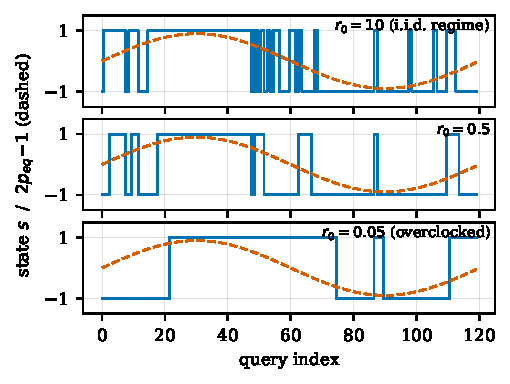
\includegraphics[width=\columnwidth]{fig_model}
\caption{Telegraph sMTJ neuron at three sampling ratios, driven by a
slowly varying firing probability (dashed). At $\rzero{=}10$ samples are
effectively i.i.d.; at $\rzero{=}0.05$ the device returns long runs of
stale state.}
\label{fig:model}
\end{figure}

\begin{figure*}[t]
\centering
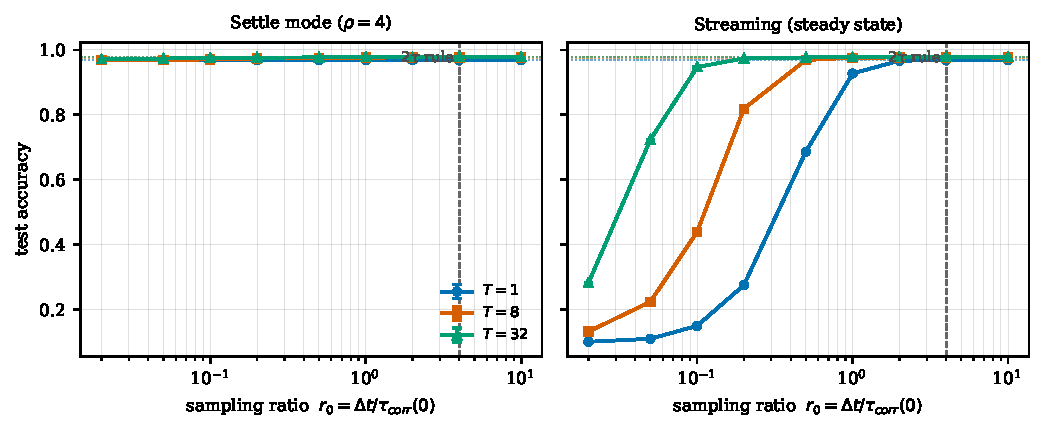
\includegraphics[width=0.9\textwidth]{fig_e2_correlation}
\caption{Accuracy vs.\ sampling ratio $\rzero$ (MNIST; mean $\pm$ std
over thermal seeds; dotted: ideal-randomness anchors; dashed vertical:
the $2\tau_d$ rule, $\rzero = 4$). \textbf{Left:} settle mode
($\rho{=}4$) is nearly rate-independent. \textbf{Right:} steady-state
streaming collapses; $T{=}1$ reaches chance below $\rzero \approx 0.05$.}
\label{fig:e2}
\end{figure*}

\subsection{Mode, not rate (E2)}
Figure~\ref{fig:e2} gives the main result. In \textbf{settle mode},
single-read accuracy is 96.90\% throughout the sweep when $\rho=4$. This
is expected: one settled read does not use the inter-read interval
(Sec.~\ref{sec:modes}), so the flat curve validates the protocol rather
than establishing a new result. The settle sweep measures the required
relaxation. Single-read accuracy is 92.9\%, 96.6\%, 96.9\%, and 96.8\% for
$\rho=1,2,4,8$, respectively. About $4\tauc$ is sufficient, whereas
$1\tauc$ is not. The cost of correlation between repeated reads is small.
At $T{=}32$ and $\rzero=0.02$, or $200\times$ faster than the rule,
accuracy decreases only from 97.73\% to 97.12\%. This residual loss follows
the standard effective-sample-size penalty of correlated averaging
\cite{sokal1997monte}: stale within-input reads reduce $T$ toward an
effective $T_{\mathrm{eff}}$, while the single-read accuracy remains high.

In \textbf{streaming mode}, steady-state accuracy collapses. Single-shot
accuracy is 96.7\% at $\rzero=2$, 92.7\% at 1, 68.6\% at 0.5, 27.5\% at
0.2, and 14.9\% at 0.1. It reaches chance (about 10\%) at
$\rzero\leq0.05$ because each input inherits the prior input's activation
state. Increasing $T$ by $32\times$ moves the 90\% crossing by roughly one
order of magnitude in $\rzero$: the crossings are approximately 0.93, 0.33,
and 0.09 for $T=1,8,32$. Even with $T{=}32$, accuracy is only 28.1\% at
$\rzero=0.02$. The bias-independent-rate variant has the same structure,
but fails at sampling ratios about $2\times$ larger: at $\rzero=0.1$,
$T{=}32$ accuracy is 53.8\%, compared with 94.7\% for the Arrhenius model.
The failure therefore comes from stale states, not from the particular rate
parameterization. The $\cosh I$ rate increase in barrier-type devices helps
because strongly driven neurons refresh faster. Fashion-MNIST shows the
same pattern: at $\rzero=0.02$, settle-mode accuracy at $T{=}32$ changes
only from 88.2\% to 87.0\%, while streaming falls to 30.2\% for $T{=}32$
and to chance for $T{=}1$.

\begin{figure*}[t]
\centering
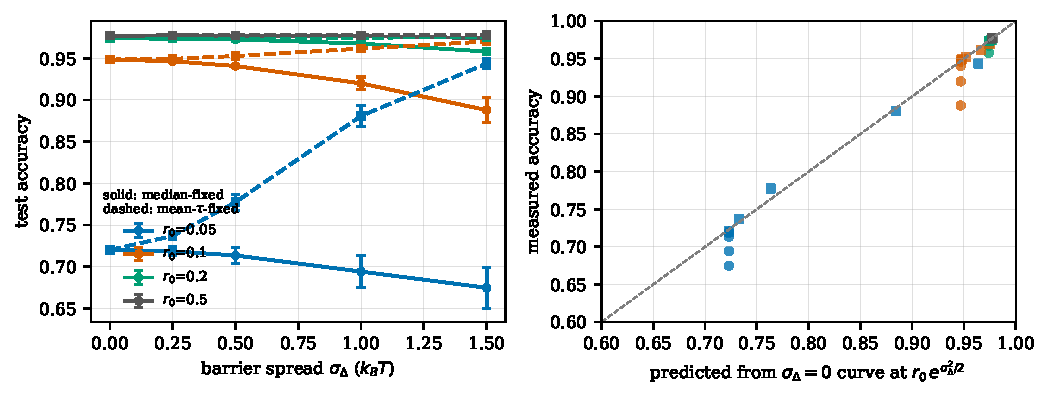
\includegraphics[width=0.9\textwidth]{fig_e3_hetero}
\caption{\textbf{Left:} apparent effect of dwell-time dispersion depends
on the fixed population statistic: median-fixed (solid) degrades;
mean-$\tauc$-fixed (dashed) appears to rescue ($T{=}32$, 5 chips,
streaming). \textbf{Right:} the rescue is the centering's uniform rate
offset in disguise: accuracy is predicted by the baseline ($\sigma_\Delta
= 0$) curve evaluated at the median-device effective ratio
$\rzero\, e^{\sigma_\Delta^2/2}$ (mean-$\tauc$) or $\rzero$ (median),
with dispersion contributing only a small residual penalty.}
\label{fig:e3}
\end{figure*}

\subsection{Centering, not dispersion, governs variability (E3)}
Because dwell time depends exponentially on barrier offset, adding
dispersion has no unique meaning until the fixed population statistic is
specified. Figure~\ref{fig:e3} shows two such cases at fixed $\rzero$. If
the \emph{median} device is fixed, accuracy declines from 72.0\% to 67.5\%
at $\rzero=0.05$ as $\sigma_\Delta$ increases from 0 to 1.5. If the
\emph{mean} correlation time is fixed, accuracy instead rises from 72.0\%
to 94.4\%. The latter improvement is primarily a centering effect. Relative
to median centering, mean-$\tauc$ centering applies the same rate multiplier
$e^{\sigma_\Delta^2/2}$ to every device, which is $3.1\times$ at
$\sigma_\Delta=1.5$. Evaluating the dispersion-free baseline in
Fig.~\ref{fig:e2} at the median-device effective ratio
$\rzero^{\mathrm{eff}}=\rzero e^{\sigma_\Delta^2/2}$ predicts the
mean-$\tauc$ result within a few points. For example,
$\rzero^{\mathrm{eff}}\approx0.15$ predicts at least 95\%, versus the
measured 94.4\%. Dispersion itself contributes a 1--5 point penalty in
both cases because the slow tail hurts more than the fast tail helps. For
overclocked streaming, device specifications should identify the central
fluctuation rate. ``Mean $\tauc$'' and ``median device'' differ by
$e^{\sigma_\Delta^2/2}$ in central rate, a larger effect than the dispersion
the specification nominally constrains~\cite{zhang2025automatic}. Although
population-level diversity can be a computational resource
\cite{mizrahi2018neural}, it is a secondary cost for this fixed network.

\begin{figure}[t]
\centering
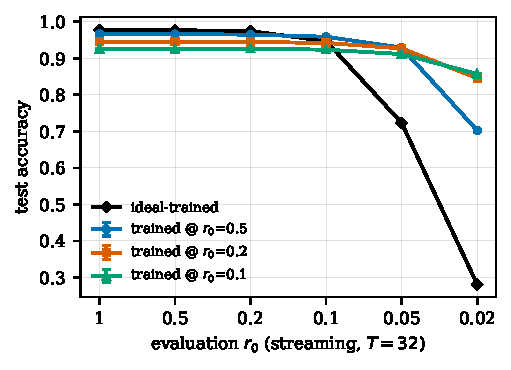
\includegraphics[width=\columnwidth]{fig_e4_training}
\caption{Correlation-aware training flattens the streaming failure curve
(steady-state, $T{=}32$; mean $\pm$ std over training and thermal
seeds).}
\label{fig:e4}
\end{figure}

\subsection{Correlation-aware training (E4)}
Networks trained with the telegraph source learn representations that are
more robust to stale states (Fig.~\ref{fig:e4}). In streaming mode with
$T{=}32$, training at $\rzero^{\mathrm{train}}=0.2$ yields 84.6\% accuracy
at $\rzero=0.02$, compared with 28.1\% for the ideal-trained baseline. The
56.5-point recovery costs 3.3 points at nominal speed: 94.5\% rather than
97.8\%. The same cost appears when both models are evaluated at the
rule-compliant $\rzero=4$, so it does not result from the chosen comparison
point. Training at $\rzero^{\mathrm{train}}=0.5$ gives a smaller
deep-overclock recovery but reduces nominal accuracy by only 1.2 points,
to 96.6\%. At $T{=}1$, training helps but does not prevent failure at the
most aggressive rates. The $\rzero^{\mathrm{train}}=0.2$ model reaches
84.1\% at $\rzero=0.2$, compared with 27.5\% for the baseline, but no
trained network avoids deep-overclock collapse at $T{=}1$. Training and
averaging therefore complement each other. This extends multi-sample,
or ``sample-aware,'' training~\cite{ghantasala2026sampling} to temporal
correlation: the network learns robustness to dependence between samples,
rather than simply benefiting from a larger sample count.

\begin{figure}[t]
\centering
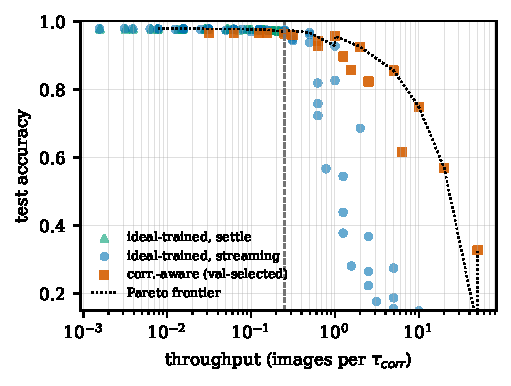
\includegraphics[width=\columnwidth]{fig_pareto}
\caption{Accuracy vs.\ physically-accounted throughput (settle mode pays
its measured $\rho{=}4$ per input; dashed vertical: best rule-compliant
single-read throughput $\rzero{=}4$). Correlation-aware points use
validation-selected training ratios.}
\label{fig:pareto}
\end{figure}

\subsection{Throughput and energy (E5)}
Settle-mode throughput cannot exceed $1/\rho=0.25$ images per $\tauc$,
regardless of read speed. Streaming has no corresponding settle limit, but
it suffers from stale-state failure. Correlation-aware training shifts that
streaming curve (Fig.~\ref{fig:pareto}). We select correlation-aware points
using only the validation split. Relative to the best rule-compliant point
at each accuracy target, the frontier is $2.0\times$ faster at 97\%
(streaming, $T{=}2$, $\rzero=2$, 97.3\%), $4.0\times$ faster at 95\%
(correlation-aware single-shot streaming at $\rzero=1$, 95.6\%), and
$8.0\times$ faster at 90\% (correlation-aware single-shot streaming at
$\rzero=0.5$, 92.5\%). These values are threshold comparisons on a finite
grid, not continuous optima. At the 90\% target, the selected point gives
up 4.4 points relative to the rule-compliant point that clears the target
(96.9\%). The comparison also assumes that readout electronics are not the
bottleneck.

For a millisecond-scale device with $\tauc\sim10$\,ms, the rule-compliant
single-read optimum is about 25 classifications per second. The frontier
supports about 100/s at at least 95\% accuracy and about 200/s at at least
90\% accuracy using the same devices. Randomness-generation energy depends
on the number of bits, $384T$ per inference. At $T{=}32$, sMTJs use
0.37\,nJ, versus 37--369\,$\mu$J for GPU or CPU PRNGs at the reported
per-bit figures~\cite{sun2026superparamagnetic}. This five-to-six-order
energy advantage does not depend on $\rzero$; overclocking turns it into
throughput by reducing the $2\tau$ wait. Another way to decorrelate samples
is to interleave $k$ devices per neuron in round-robin order. That increases
each device's effective sampling interval by $k$, moving along the same
accuracy-versus-$\rzero$ curves at $k\times$ the device area.

\section{Discussion}
\label{sec:discussion}
\textbf{Design guidance.} The $2\tau_d$ rule remains appropriate for TRNG
bitstream certification~\cite{vodenicarevic2017low,sun2026superparamagnetic},
but classification inference depends on workload. In settle-mode pipelines,
devices can be read very quickly once each input receives about $4\tauc$ of
relaxation; that settle time becomes the throughput cost. Streaming has a
real stale-state boundary. Correlation-aware training and sample averaging
move that boundary, whereas fabrication uniformity does not. Specifications
for overclocked devices should also identify the population statistic held
fixed. Because dwell time depends exponentially on barrier height, the
mean-$\tauc$ and median-device conventions differ by
$e^{\sigma_\Delta^2/2}$ in central rate. Finally, at matched $\tauc$,
barrier-type devices tolerate overclocking better than bias-independent-rate
devices because strong inputs also refresh their neurons faster.

\textbf{Limitations.} This simulation uses an idealized two-state model. It
does not include read disturb, retention drift, or $1/f$ noise
\cite{sun2026superparamagnetic}; it also uses small MLPs and MNIST-class
benchmarks. The streaming experiments assume consecutive inputs are
uncorrelated. Correlated input streams, such as video, could interact with
staleness differently. The Pareto gains are threshold values on a finite
grid, not continuous optima. Testing fabricated arrays such as the
instrumented systems in~\cite{singh2024cmos}, then extending the analysis to
convolutional networks and temperature drift, would test these conclusions
under more realistic conditions.

\section{Conclusion}
Violating the sMTJ sampling rule has different consequences in the two
operating modes. Batch-style inference can sample $200\times$ faster than
the rule with less than one percentage point of loss, provided each input
receives a measured settle of about $4\tauc$. In steady-state streaming,
stale device states drive accuracy to chance. Fabrication dispersion does
not remedy that failure; its apparent benefit mainly reflects the chosen
centering convention. Correlation-aware training recovers much of the loss.
Treating sampling ratio as a design variable turns autocorrelation into
throughput, reaching $2$--$8\times$ the rule-compliant optimum depending on
the accuracy target while retaining the roughly $10^6$-fold random-bit
energy advantage of p-bit hardware.

\section*{Acknowledgment}
This work was developed with generative AI assistance (Anthropic Claude;
OpenAI Codex) under the author's direction, spanning simulator and
experiment implementation and preparation of the manuscript, including
drafting, revision, and its related-work survey; an AI-assisted
adversarial review was used to stress-test the methodology before
submission. The author set the research questions and design, validated
the results, and takes full responsibility for the content. The author
thanks the UCSB Summer Research Academy for introducing him to
probabilistic computing.

\bibliographystyle{IEEEtran}
\bibliography{refs}

\begin{IEEEbiographynophoto}{Manan Gupta}
is a senior at The Harker School, San Jose, CA, USA. His research
interests include probabilistic and stochastic computing, machine
learning systems, and energy-efficient AI hardware. He has conducted
independent research in machine-learning classification and quantum
computing through programs at UC Irvine and UC Santa Barbara, where he
studied probabilistic computing with stochastic magnetic tunnel
junctions. He is a USACO Silver division competitor and a contributor to
open-source software projects.
\end{IEEEbiographynophoto}
%% TODO: replace with \begin{IEEEbiography}[{\includegraphics[width=1in,height=1.25in,clip,keepaspectratio]{author_photo.png}}]{Manan Gupta} ... once photo is added

\EOD

\end{document}
